% !TEX options=--shell-escape

\documentclass[11pt]{article}

\usepackage{geometry}
\usepackage[hidelinks, colorlinks=true, linkcolor=blue, citecolor=blue]{hyperref}

% APA citation style
\usepackage{natbib}
\usepackage{apalike}

\usepackage{setspace} % line spacing

\usepackage{bm}

% Paragraph indentation (first line)
\setlength{\parindent}{0em}
% Paragraph spacing
\setlength{\parskip}{.7em}

\usepackage{caption}

% Names of subsections and figures in cross-references with \autoref{}
\renewcommand*{\sectionautorefname}{Section}%
\renewcommand*{\subsectionautorefname}{Section}%
\renewcommand*{\figureautorefname}{Fig.}%

\usepackage{textcomp} % fancy symbols in text mode (e.g. right arrow)
\newcommand{\textapprox}{\raisebox{0.5ex}{\texttildelow}}

% For images
\usepackage{graphicx, rotating}

% Center caption text for images
\usepackage[justification=centering]{caption}

% styling of examples (use like: \Example{title text}{text}{label}), including their counting and referencing with \autoref{label}
\newcounter{examplecount}
\newcommand*{\examplecountautorefname}{E\kern-0.3em}
\newcommand{\Example}[3]{
	\vspace{0.4cm}\\
	\refstepcounter{examplecount}
	\hspace*{1cm}\parbox{12cm}{(E\arabic{examplecount}) #1}

	\hspace*{1.5cm}\parbox{12cm}{\texttt{#2}\label{#3}}\\[0.4cm]
}

\usepackage{listings}
\lstset{
  columns=flexible,
  basicstyle=\ttfamily,
  mathescape=true,
  escapeinside=||
}

\usepackage[none]{hyphenat}

\title{\LARGE Introduction to Discourse Analysis -- Assignment 2 \\ Task 5}
\date{}
\author{}

\begin{document}

\maketitle

\,
\vspace{-5em}

%%%%%%%%%%%%%%%%%%%%%
% total words: 1549 + 102 - 5 - 8 - 7 - 2 - 10 - 6 %
%%%%%%%%%%%%%%%%%%%%%

% INSTRUCTIONS
% In completing the tasks, you are expected to demonstrate your understanding of relevant theoretical concepts and frameworks (review section), your ability to apply that understanding to a specific case/situation and relevant academic writing skills. 
% In the theoretical section, feel free to draw on data from the literature to illustrate the various theoretical points. 
% Likewise, in the analysis section, feel free to draw on examples from the literature to support further your claims.

% TASK 5
% Marcia’s turn in lines 21-23 in the extract below appears to be an account. 
% Yet, it is not obvious what it is an account of. 
% Describe the sequential organisation of talk in the extract and show how the account comes about.
% The question is about how the speaker ends up having to utter an account.

% terms: hedge, false start, warrant, dispreferred FPP

% TRANSCRIPTIONS:
% - .hhh: inbreath
% - hhh: outbreath
% - =: continuous transition from one TCU to another
% - {}
% - []: overlapping talk
% - (.): brief interval
% - word-: cut-off

\section*{Introduction}{
	% CA about actions
	% - CA (fathers Schegloff, Sacks) about social actions in speaking, not about speaking itself
	Conversation analysis 
	% helps analyse social interactions by relating the surface form of talk and underlying actions
	approaches conversations as social interactions, relating the surface form of talk and the underlying actions of participants.
	% i analyse short conversation using sequential organisation, using preference to analyse how potentially socially problematic actions (asking for a big favour, and refusing to help) are realised in it
	In this work, I look at a short conversation, applying the \textit{sequential organisation} approach. In particular, I use the concept of \textit{preference} to analyse how potentially socially problematic actions -- asking for a big favour, and refusing to help -- are realised.
}

% 736
\section*{Theoretical background}{
	% - speaking is mostly sequential; seq. org. about how actions are ordered in interaction (conversation), how an action influences what comes next, eventually constructing orderly sequences of talk
	Sequential organisation explores how actions (requesting, inviting, telling...) are ordered when they surface in conversation; how an action influences successive actions so that orderly sequences of talk are created.
    
    % - notion of ``conditional relevance'': an action makes a certain next action(s) relevant (or even expected), e.g. a question makes an answer be the relevant next action.
    \textit{Conditional relevance} \citep{Schegloff_1968} describes how one action makes certain next action(s) relevant (suitable, or even required if the talk is to proceed orderly), e.g. a question inviting an answer.
    % - hence adjacency pairs: basic units of seq. org. \citep{Schegloff_1973}. defined by \citet[p.~64]{Sidnell_2010} as: ``Adjacent. Produced by different speakers. Ordered as a first pair part (FPP) and a second pair part (SPP). Typed, so that a particular FPP provides for the relevance of a particular SPP (or some delimited range of SPPs)''
    Thus, long sequences consist of basic units -- \textit{adjacency pairs}; defined by \citet[p.~64]{Sidnell_2010} as pairs of utterances:
    \begin{enumerate}
    	\item Adjacent
    	\item Produced by different speakers
    	\item Ordered as a first pair part (FPP) and a second pair part (SPP)
    	\item Typed, so that a particular FPP provides for the relevance of [occasions] a particular SPP (or some delimited range of SPPs)
    \end{enumerate}
    The \textit{type} of a pair can be e.g. greeting-greeting or question-answer, an example adjacency pair of the latter type being:
    % - example adj. pair \Example{from \citet[p.~107]{Liddicoat_2007}}{John: What time' s it? \\Betty: Three uh clock.}{adj-pair}
    \Example{from \citet[p.~107]{Liddicoat_2007}}{John: What time' s it? \\Betty: Three uh clock.}{adj-pair}
    %   - the two lines are FPP and SPP, adjacent, produced by different speakers, and <<typed>> -- FPP is a question, which makes relevant an SPP of type answer
    %   - also note that speaker 1 gives speaker 2 space to react (in this case they stop speaking), or else they can't expect an SPP to occur!
    Notice too how John stops speaking, giving Betty space to produce an SPP (otherwise, there would be no interaction!)
    %   - also, an FPP requires a relevant SPP! if Betty stayed silent, John would likely repeat his question (unless he'd interpret the silence a relevant response)
    and Betty's producing of a \textit{relevant} SPP -- if she stayed silent, John could repeat/restate his question (his FPP \textit{requiring} an SPP) or interpret Betty's silence as a response.
    % - by producing a matching SPP, speaker 2 shows they understood the FPP, and a conversation continues orderly
    By producing a matching SPP, Betty also shows understanding of the preceding FPP and the conversation continues smoothly.

    % - an FPP doesn't occasion one particular SPP (and a meaningful reaction can also be non-verbal, e.g. silence or in \autoref{adj-pair} Betty showing John her wristwatch)
    Importantly, an FPP can occasion many possible SPPs (including non-verbal actions, e.g. Betty showing John her wristwatch),
    % - BUT given an FPP, not all relevant SPPs may be equally valued: ``some responses are problematic for social relationships, while others are not'' \citep[p.~111]{Liddicoat_2007}
    but they are often unequally valued: ``some responses are problematic for social relationships, while others are not'' \citep[p.~111]{Liddicoat_2007}.
    % - we can talk of usual/typical reactions as preferred (e.g. Betty's answer in \autoref{adj-pair}), whereas less normal/socially appropriate reactions are termed dispreferred (e.g. Betty answering ``I don't know'' instead).
    Usual/unsurprising reactions are termed \textit{preferred} (e.g. the answer in \autoref{adj-pair}); less socially appropriate/normal are \textit{dispreferred} (e.g. if Betty answered ``I don't know'').
    % - typically, the participants are aware of the social norms which make certain reactions preferred or dispreferred, and make the two surface differently in their speaking:
    Aware of social norms, participants typically treat the two types differently in speaking.
    % - preferred reactions, such as accepting an invitation, typically surface as short and immediate, like A's accepting in \autoref{pref}
    Preferred reactions (e.g. accepting an invitation) surface as short and immediate:
    \Example{from \citet[p.~58]{Casson_1981}}{B: Why don't you come up and see me some[times\\A: \hspace{18.5em}[I would like to}{pref}
    % - dispreferred reactions, on the other hand, surface in ways that mitigate their potential negative social impact, see 
    while dispreferreds surface in ways that mitigate potential negative social impact:
    \Example{adapted from \citeauthor[p.~110]{Liddicoat_2007}}{Harry: I don' have much tuh do on We:nsday.\\\phantom{.}~\hspace{2.9em}(.)\\\phantom{.}~\hspace{2.9em}w' d yuh like tuh get together then.\\\phantom{.}~\hspace{2.9em}(0.3)\\Joy: \ \ huh we::llhh I don' really know if yuh see\\\phantom{.}~\hspace{2.9em}i' s a bit hectic fuh me We:nsday yih know}{dispref}
    % - the rejection of the invitation is nearly not as overt as the acceptance. it comes with a delay of 0.3s, the hesitant ``we::ll'' with out-breathing, with hedges (``I don' really know'' and ``\textbf{a bit} hectic''), and explanations (accounts) for the refusal rather than a clear refusal itself. these signs are termed dispreferrence markers -- compare with shortness, overtness and lack of account as possible preferrence markers.
    Joy's rejection is weak, comes with 0.3s delay, a hesitant ``we::ll'', hedges (``I don' really know'', ``\textbf{a bit} hectic''), and explanations (accounts) rather than a clear refusal. These common signs -- \textit{dispreference markers} -- contrast with the shortness, overtness and lack of account (\textit{preference markers}) in \autoref{pref}.
    
    % - as \citet{Liddicoat_2007} points out, not just SPPs, but also FPPs can be dispreferred, e.g. requests, which are then ``held back as later topics'' and ``accompanied by accounts and mitigations, which occur before the request itself'' -- i.e. dispreferrence markers, as seen in XXX, following Jim's previous (preparatory) explanations of his pitiful situation:  he provides a lengthy account and then makes the actual request in an indirect way using ``was wondering'' and ``could''.
    Importantly, FPPs can be dispreferred too (e.g. requests) and are then ``held back as later topics'' and ``accompanied by accounts and mitigations, which occur before the request itself'' \citep[p.~122]{Liddicoat_2007}:
    % - \Example{from \citet[p.~122]{Liddicoat_2007}}{Jim: well my car has broken down an they don' know\\\phantom{.}~\hspace{2.1em}if it will be fixed by then an' I w' z wondering\\\phantom{.}~\hspace{2.1em}if I c' d borrow your car.}{dispref-fpp}
    \Example{from \citeauthor[p.~122]{Liddicoat_2007}}{Jim: well my car has broken down an they don' know\\\phantom{.}~\hspace{2.1em}if it will be fixed by then an' I w' z wondering\\\phantom{.}~\hspace{2.1em}if I c' d borrow your car.}{dispref-fpp}
    Following his previous (preparatory) explanations of the pitiful situation, in the first 2 lines of \autoref{dispref-fpp} Jim provides a lengthy account before wording the actual request indirectly, using ``was wondering'' and ``could''.

    % SPP can become FPP
    When moving beyond single adjacency pair, the SPP of one pair can become the FPP of the next pair, giving rise to longer action sequences. 
    % pairs can also be expanded to create longer sequences: pre-, post- and inserts. all of these can be also long sequences!
    Alternatively, a pair can be expanded by adding an element before (pre-expansion), between (insert-expansion) or after (post-expansion) the FPP and SPP. Indeed, the added element can itself be a longer sequence.
    % pre-expansions: w.r.t. preference, a dispreferred tends FPP e.g. the main request sequence tends to be preceded by a pre-sequence which checks if preconditions are met (e.g. if the person needs their car atm), and which may make the request more relevant (and less dispreferred) by perhaps explaining the reasons for it.
    With regard to preference, a pre-sequence may, as already hinted, precede a dispreferred FPP and check if some preconditions are met (e.g. if the other person needs their car right now) and/or make the request more relevant (less dispreferred) by perhaps first explaining the situation.
    % insert-expansions: actions before producing SPP -- whether clarifying the FPP or requesting further information upon which an SPP depends
    An insert-sequence can be employed e.g. before a dispreferred SPP to mitigate the contrast with the FPP (similar to delaying the SPP using a pause like in \autoref{dispref}).
    % post-expansions: Q-A-assessment (minimal vs non-minimal)
    Finally, a post-expansion adds to the pair -- either in a \textit{minimal} way which effectively closes the sequence (such as adding ``Right, okay'' in \autoref{adj-pair}), or in a \textit{non-minimal} way where the added ``third pair part'' itself becomes an FPP and makes some next action relevant.
}

\section*{Analysis}{
	% At a high level, the data (shown in \autoref{fig:data-marked}) is a short call, whereby Donny calls Marcia and starts describing how his car broke down in Glen while he needs to be in Brentwood -- supposedly fairly soon, and he supposedly needs a new car to get there. Marcia interrupts him and explains how she would love to help, but she needs to leave for some duties very soon (supposedly using her car). Then, Donny closes the talk very quickly, planning to call someone else (supposedly to borrow a car from them).
	The data (\autoref{fig:data-marked}) is a short call; Donny calls Marcia, starts describing how his car broke down, he needing to be somewhere else (supposedly soon, and hence needing another car). Marcia reacts, explaining she would love to help but she herself has to go (supposedly using her car). Then, Donny concludes he would call someone else and closes the conversation quickly.

	\begin{figure}[h!tb]
		\centering
		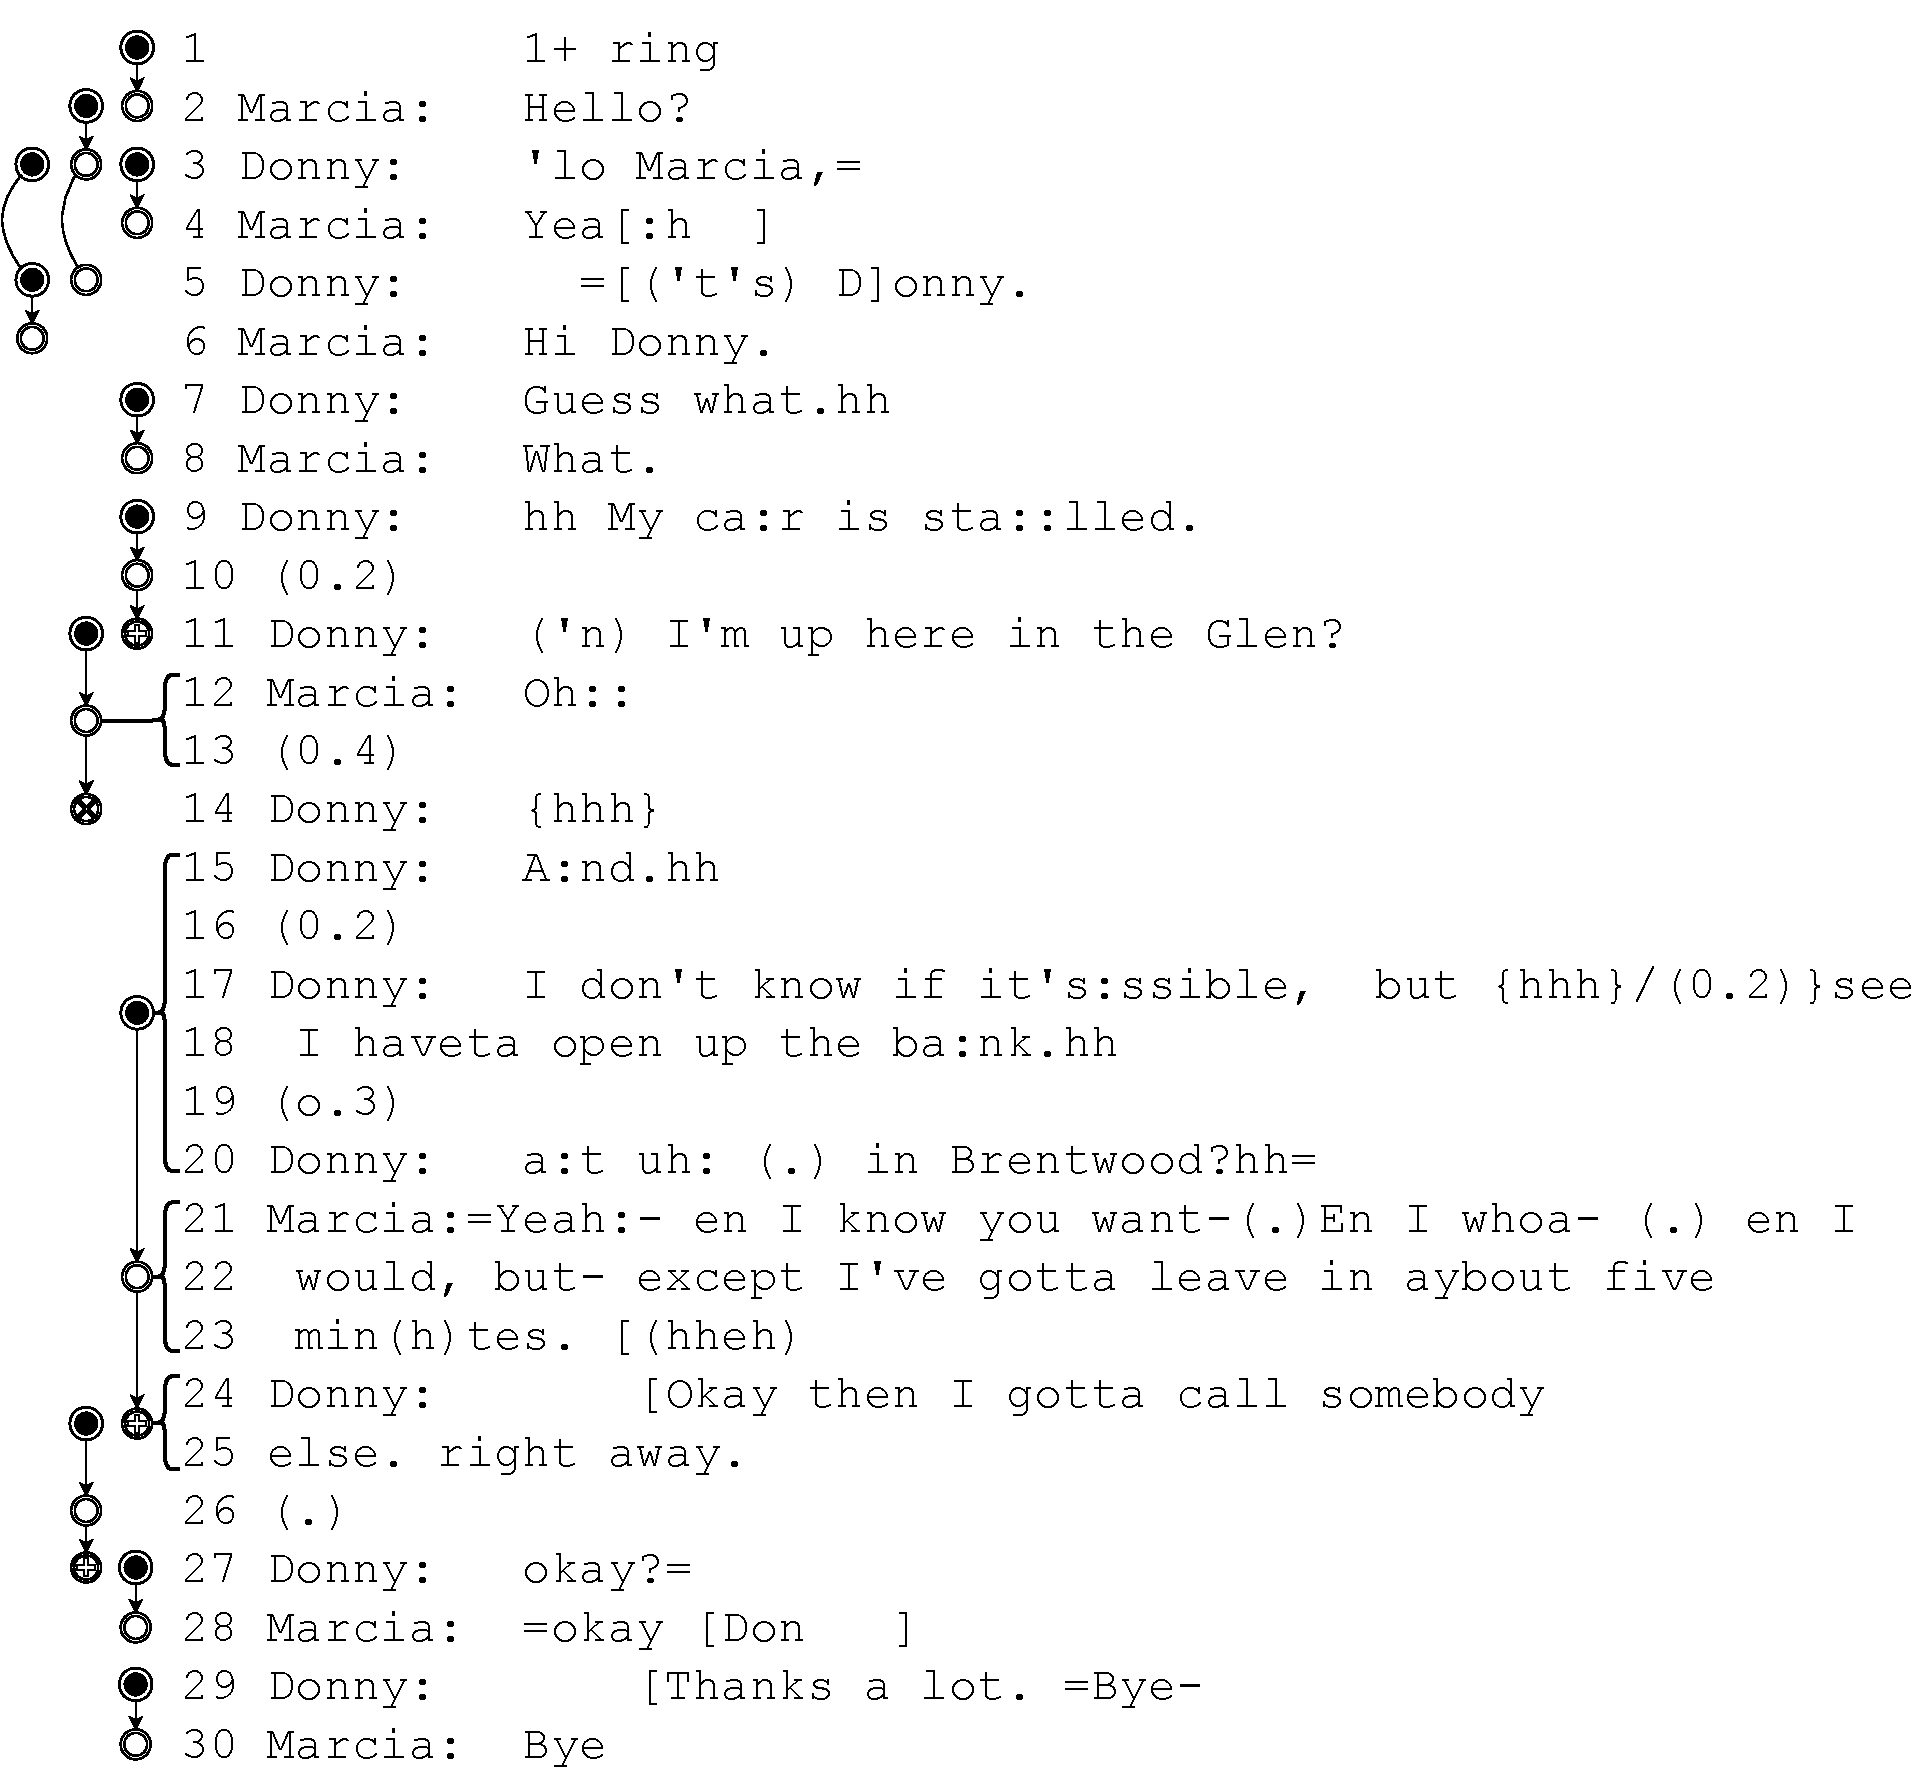
\includegraphics[width=\columnwidth]{../data-marked.pdf}
		\caption{The data; sequence organisation marked on the left. Black circles mark FPPs, blank circles SPPs; $\boldsymbol{\mathbf{\otimes}}$ and $\boldsymbol{\mathbf{\oplus}}$ mark minimal/non-minimal post-expansions, respectively. Where connected by lines without arrowheads (L3,5), and where curly braces are used (e.g. L21-23), it means multiple lines forming one pair part.}
		\label{fig:data-marked}
	\end{figure}

	% I will now chronologically step through and describe the excerpt's sequential organisation, particularly with respect to Marcia's account (L21-23). (All adjacency pairs I also marked directly in \autoref{fig:data-marked}.)
	I chronologically step through and describe the excerpt's sequential organisation, particularly with respect to Marcia's reaction (L21-23). (All adjacency pairs marked also in \autoref{fig:data-marked}.)

	L1-2 is a typical \textit{summons-answer} pair \citep[p.~126]{Liddicoat_2007}, a pre-sequence enabling a conversation to begin. Notice Donny's non-verbal action (L1) -- face-to-face, it could be ``Hey, Marcia!''.
	% L2 as FPP inquires who the caller is, upon which Donny identifies himself (L3+5).
	As an FPP, L2 asks the caller to identify themselves, and Donny does that in L3\&5.
	% Marcia's interruption (L4) is not clear, but could signal that she recognised Donny already from L3, or that she confirms her identity after Donny addressed her by name in L3. Either way, Donny was not finished and ends his FPP in L5.
	Marcia's interruption (L4) I find ambiguous -- she could signal recognition of Donny, or confirm her identity after Donny addressed her. Either way, Donny continues, finishing in L5.
	% L3+5 with L6 is a classical greeting-greeting pair which ends the opening section of the call. Note that this is a short form; a common, longer one would also add ``how are you?'' to the greetings, potentially lengthening the call opening with further chit-chat.
	The standard greeting-greeting pair (L3\&5, L6) ends the call's opening. Notice the brief form; often, ``how are you?'' would be added.

	After the opening, which can be viewed as a pre-sequence, Donny pushes the conversation forward with a further pre-sequence (L7) -- a \textit{pre-telling} \citep[p.~136]{Liddicoat_2007} pair: Signalling he has something to tell and Marcia giving a ``go-ahead'' (L8).
	Then, Donny's telling unravels (L9-L20), which will turn out to be another pre-sequence.
	Donny's FPP (L9) announces unfortunate news, inviting a sympathetic SPP, but silence follows (L10) -- attributable to Marcia's lack of relevant response.
	Hence, Donny post-expands (L11), introducing further bad news, making a sympathetic reaction even more relevant (or even required).
	To L11 as an FPP, Marcia finally responds (L12-13), but her ``Oh::'' I see merely as signalling receipt of new information (see detailed analysis of ``oh'' by \citet{Heritage_1984}). Then, Marcia goes silent (L13), not taking further stance or assessing Donny's situation (the silence can also be Donny giving her space to continue).
	Eventually,	Donny accepts Marcia's position; closes the telling sequence by minimally post-expanding (L14 -- merely an outbreath) before moving on.

	Across L15-20, Donny starts the conversation's main sequence (following the pre-request telling), putting forward his request. His FPP's dispreferredness is heavily marked by: length, hesitations (L15, breathing (L17), tokens ``a:t u:h'' (L20)), pauses (L16, 17, 19, 20), only slowly moving to the point, placing it after a hedge (``I don't know if it's:ssible'') and a warrant (``see I haveta open up the ba:nk''). Without directly requesting Marcia's car, the request comes across clearly and Marcia has to react (L21-23).

	Marcia's reaction is also dispreferred (a refusal) and heavily marked: with short pauses, and hesitations where she stops to repair her talk (the \verb|word-| patterns (L21-22)). Starting with sympathetic ``Yeah:'' -- acknowledging Donny's pitiful situation; then confirming she understands the request (``en I know you want-''); showing willingness to help (``en I would''); before finally providing an account for not helping (``I've gotta leave in aybout five min(h)tes'').

	Without directly refusing, Marcia's SPP is understood by Donny; he non-minimally post-expands (L24-25), acknowledging Marcia's refusal (``Okay then'') and mitigating its dispreferredness by outlining contingency plans (to call someone else). The post-expansion is also an FPP -- summarises the main sequence and starts a typical \textit{sequence-closing sequence}, which \citep[p.~168]{Liddicoat_2007} normally consists of:
	\begin{enumerate}
		\item summary/assessment proposing to close,
		\item go-ahead signal for closing,
		\item final turn, closing the sequence.
	\end{enumerate}
	However, Marcia uncooperatively stays silent (L26), upon which Donny post-expands (L27), repeating his suggestion-to-close more explicitly (``okay?''). To this FPP, Marcia responds quickly with the preferred ``go-ahead'' SPP (L28). Then, Donny readily closes the conversation with a typical closing pair (L29-30).
}

\section*{Overall view and conclusions}{
	Through sequential organisation analysis, we saw the conversation unrolling in pre-sequences (opening~$\rightarrow$~pre-telling~$\rightarrow$~telling), preparing the ground for the main request sequence.
	Throughout, Marcia is minimalistic and uncooperative -- perhaps because being busy, but I also interpret it as early signals to Donny: 
	Figuring out that his speaking is only a pre-sequence, she anticipates \textit{some} request and signals unavailability to help.
	Donny ignores these signals, pushes on, until making the actual request.
	At that point, Marcia cannot just signal anymore and refuses openly.

	The framework of \textit{preference} lets us see how -- although both participants are in a hurry -- the strong social norms make them present the dispreferred request and refusal in characteristic, elongated ways.
}

\bibliographystyle{apalike}
\bibliography{B083350.bib}

\clearpage
\section*{Appendix -- the raw data}{
	\textbf{Marcia and Donny, stalled}
\begin{lstlisting}
1           1+ ring
2 Marcia:   Hello?
3 Donny:    'lo Marcia,=
4 Marcia:   Yea[:h  ]
5 Donny:      =[('t's) D]onny.
6 Marcia:   Hi Donny.
7 Donny:    Guess what.hh
8 Marcia:   What.
9 Donny:    hh My ca:r is sta::lled.
10 (0.2)
11 Donny:   ('n) I'm up here in the Glen?
12 Marcia:  Oh::
13 (0.4)
14 Donny:   {hhh}
15 Donny:   A:nd.hh
16 (0.2)
17 Donny:   I don't know if it's:ssible,  but {hhh}/(0.2)}see
18  I haveta open up the ba:nk.hh
19 (o.3)
20 Donny:   a:t uh: (.) in Brentwood?hh=
21 Marcia:=Yeah:- en I know you want-(.)En I whoa- (.) en I
22  would, but- except I've gotta leave in aybout five
23  min(h)tes. [(hheh)
24 Donny:       [Okay then I gotta call somebody
25 else. right away.
26 (.)
27 Donny:   okay?=
28 Marcia:  =okay [Don   ]
29 Donny:       [Thanks a lot. =Bye-
30 Marcia:  Bye
\end{lstlisting}
}

\end{document}
